
下面把 $\mathfrak H_X$
与 $\mathfrak H_a$、$\mathfrak H_d$ 胶合。
为此，先把 $\mathfrak H_X$
与下文将构造的另一个同伦等价
$\mathfrak J$ 复合。

首先取 $[0,1]_r\times C(L'_1,\lambda'_1)$
的一个模型。
再由命题~\ref{prop:7-2-190}
得到 $[0,1]^2\times C(L'_1,\lambda'_1)$
的模型 $\widehat{\mathfrak C}_Y(L'_1)$，
使
\[
\begin{aligned}
\bigl(\widehat{\mathfrak C}_Y(L'_1)\bigr)_{r=0}
&=C([0,1]_s\times L'_1,\lambda'_1)
=\bigl(\widehat{\mathfrak C}_Y(L'_1)\bigr)_{r=1},\\
\bigl(\widehat{\mathfrak C}_Y(L'_1)\bigr)_{s=s_0}
&=C(L'_1,\lambda'_1)^{[0,1]_r}.
\end{aligned}
\]

\begin{lemma}{7.2.342}\label{lem:7-2-342}
存在滤过 $A_{n',K'}$ 同伦等价\translatornote{原书第二个映射的源写作带帽的
$\widehat{\mathfrak C}_X^{s=s_0}(L'_1)$；
这里按 (7.2.339.2) 所定义的
$s=s_0$ 限制模型写作
$\mathfrak C_X^{s=s_0}(L'_1)$。
图式 7.2.29 亦将其写成
$(\widehat{\mathfrak C}_X(L'_1))_{s=s_0}$。}
\[
\begin{aligned}
\mathfrak J\colon\;&
\widehat{\mathfrak C}_X(L'_1)
\longrightarrow\widehat{\mathfrak C}_Y(L'_1),\\
\mathfrak J^{(s=s_0)}\colon\;&
\mathfrak C_X^{s=s_0}(L'_1)
\longrightarrow
\bigl(\widehat{\mathfrak C}_Y(L'_1)\bigr)_{s=s_0},
\end{aligned}
\]
它们满足以下条件：
\begin{equation}
\operatorname{Eval}_{s=s_0}\circ\mathfrak J
=\mathfrak J^{(s=s_0)}
\circ\operatorname{Eval}_{s=s_0},
\tag{7.2.343.1}\label{eq:7-2-343-1}
\end{equation}
\begin{equation}
\mathfrak J\circ\operatorname{Incl}
=\operatorname{Incl}\colon
C(L'_1,\lambda'_1)
\longrightarrow\widehat{\mathfrak C}_Y(L'_1),
\tag{7.2.343.2}\label{eq:7-2-343-2}
\end{equation}
且图式~\ref{diag:7-2-28} 交换。

\par\medskip\noindent\begin{minipage}{\textwidth}
\centering
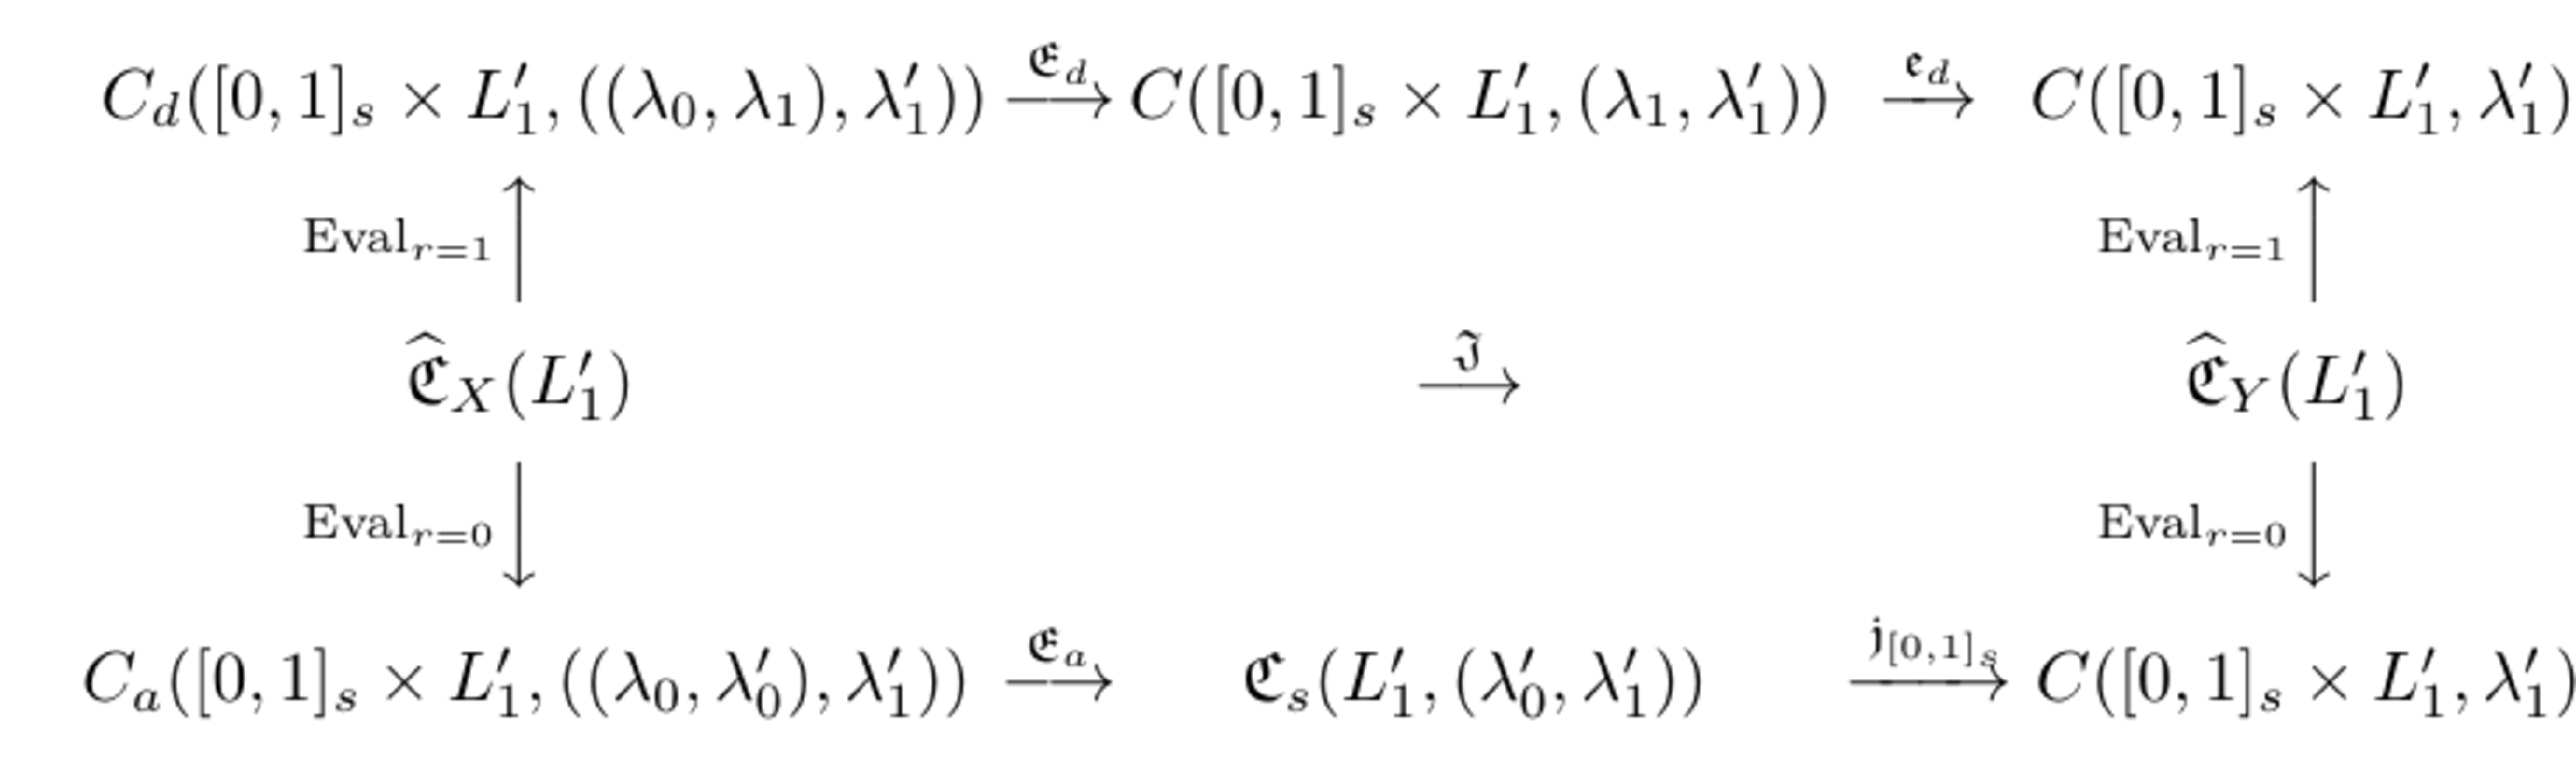
\includegraphics[width=\textwidth]{chapters/ch07-transversality/figures/phys-572-diagram-7-2-28-math-final-crop.png}
\par{\renewcommand{\thefigure}{7.2.28}\refstepcounter{figure}
\normalfont\bfseries 图式~\thefigure\label{diag:7-2-28}}
\end{minipage}\par\medskip
\end{lemma}

图式~\ref{diag:7-2-28}
与 (7.2.343) 共同推出
\begin{equation}
\operatorname{Incl}_r
=\mathfrak J^{(s=s_0)}\circ\operatorname{Incl}_r
\colon C(L'_1,\lambda'_1)
\longrightarrow
\bigl(\widehat{\mathfrak C}_Y(L'_1)\bigr)_{s=s_0}.
\tag{7.2.344}\label{eq:7-2-344}
\end{equation}
它们还推出下列交换图式：

\par\medskip\noindent\begin{minipage}{\textwidth}
\centering
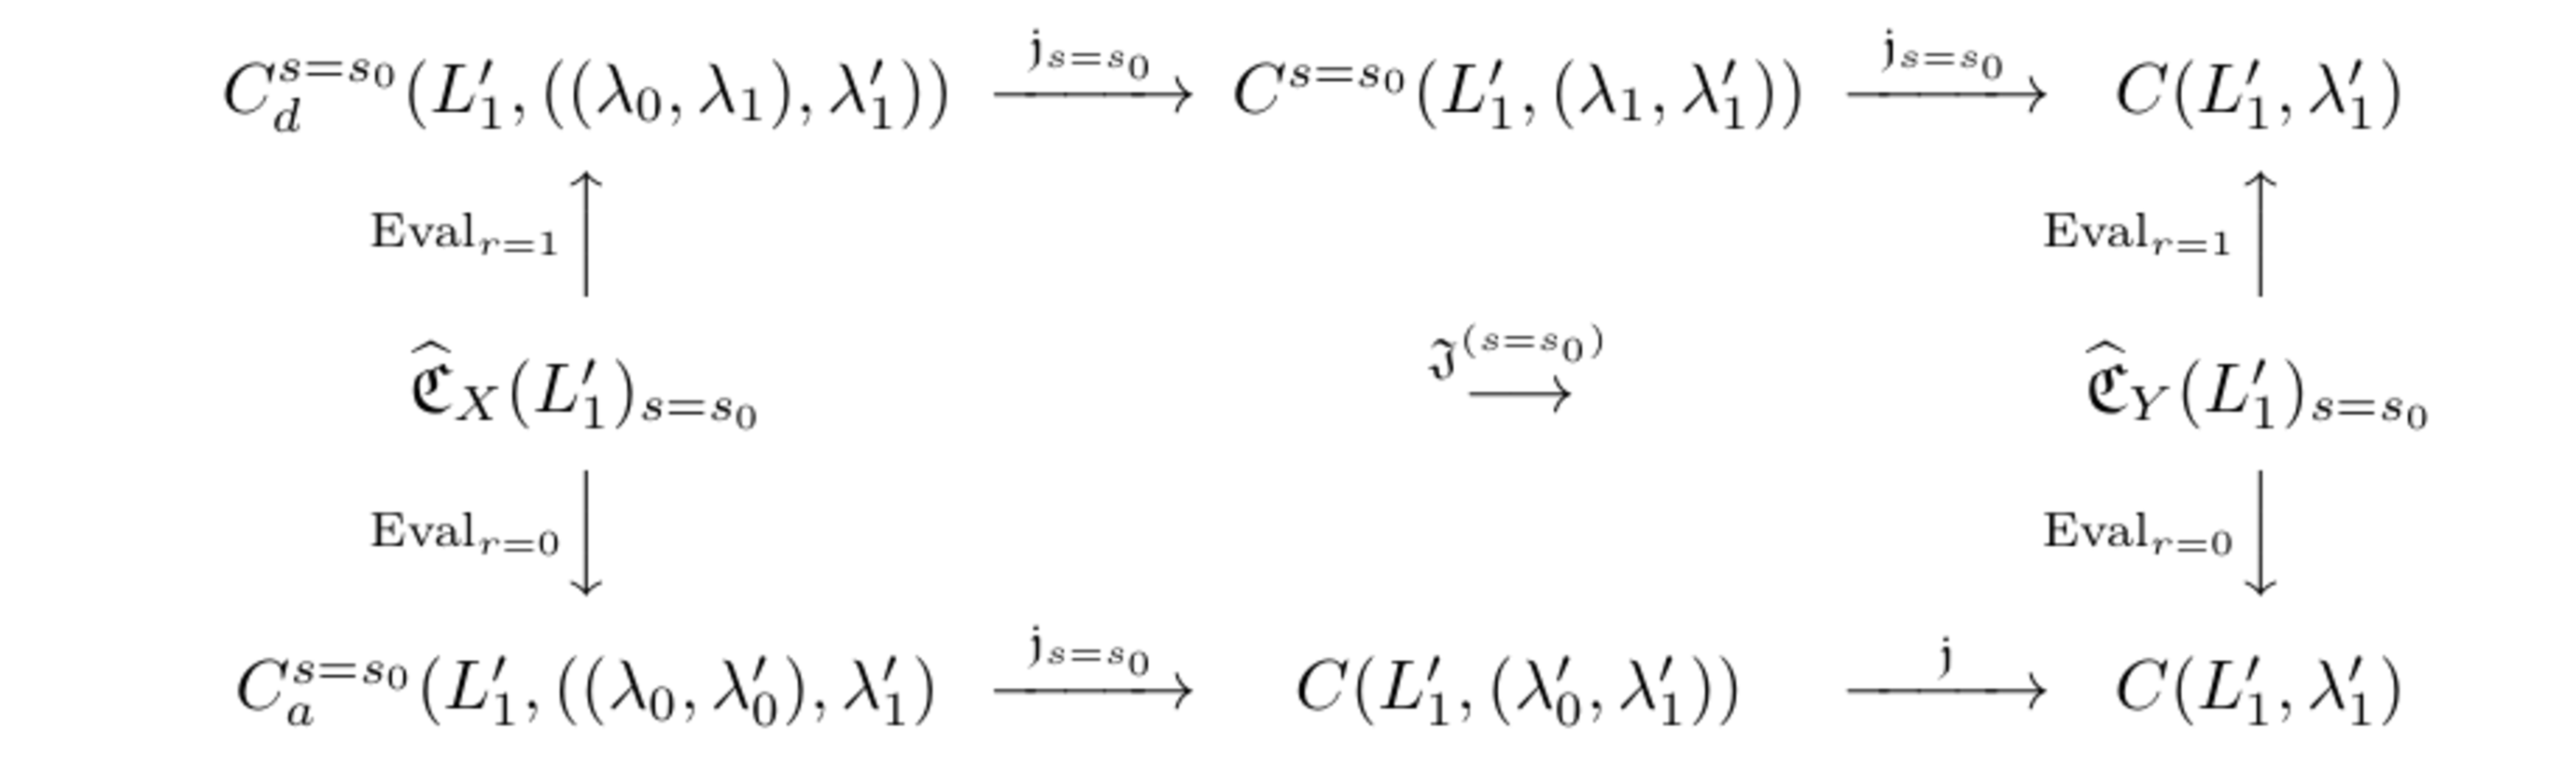
\includegraphics[width=\textwidth]{chapters/ch07-transversality/figures/phys-572-diagram-7-2-29-math-final-crop.png}
\par{\renewcommand{\thefigure}{7.2.29}\refstepcounter{figure}
\normalfont\bfseries 图式~\thefigure\label{diag:7-2-29}}
\end{minipage}\par\medskip

\noindent\textbf{引理~\ref{lem:7-2-342} 的证明。}
先用定理~\ref{thm:7-2-176}
构造 $\mathfrak J^{(s=s_0)}$，
使图式~\ref{diag:7-2-29} 交换，
且 (7.2.344) 成立。
再用命题~\ref{prop:7-2-312}
构造 $\mathfrak J$。
令
\[
C'_0=C(L'_1,\lambda'_1),\qquad
C'=\widehat{\mathfrak C}_X(L'_1),\qquad
\widehat{\mathfrak C}
=\widehat{\mathfrak C}_Y(L'_1).
\]
并定义
\[
\begin{aligned}
\mathfrak h&=\operatorname{Incl},\\
\mathfrak H^{r=0}
&=j_{[0,1]_s}\circ\mathfrak E_a
\circ\operatorname{Eval}_{r=0},\\
\mathfrak H^{r=1}
&=\mathfrak e_d\circ\mathfrak E_d
\circ\operatorname{Eval}_{r=1},\\
\mathfrak H^{s=s_0}
&=\mathfrak J^{(s=s_0)}
\circ\operatorname{Eval}_{s=s_0},\\
\mathfrak H_0
&=\operatorname{Incl}\colon
C(L'_1,\lambda'_1)
\longrightarrow\widehat{\mathfrak C}_Y(L'_1).
\end{aligned}
\]

下面验证 (7.2.313)。
由 (7.2.305.4)、(7.2.305.3) 得
\[
\operatorname{Eval}_{s=s_0}
\circ\mathfrak H^{r=0}
=j\circ j_{s=s_0}\circ
\operatorname{Eval}_{s=s_0}
\circ\operatorname{Eval}_{r=0}.
\]
另一方面，
图式~\ref{diag:7-2-29} 的交换性给出
\[
\operatorname{Eval}_{r=0}
\circ\mathfrak H^{s=s_0}
=j\circ j_{s=s_0}\circ
\operatorname{Eval}_{s=s_0}
\circ\operatorname{Eval}_{r=0}.
\]
所以在 $r=0$ 时，
(7.2.313.1) 得证。

再由 (7.2.333.4)、(7.2.333.5)，
计算得\translatornote{以下双
$j_{s=s_0}$ 保留源式；
它与 (7.2.335.1) 的同名复合
有同一型别疑点，
目前不删除其中任何一重。}
\[
\operatorname{Eval}_{s=s_0}
\circ\mathfrak H^{r=1}
=j_{s=s_0}\circ j_{s=s_0}
\circ\operatorname{Eval}_{s=s_0}
\circ\operatorname{Eval}_{r=1}.
\]
另一方面，由图式~\ref{diag:7-2-29}
的交换性，
\[
\operatorname{Eval}_{r=1}
\circ\mathfrak H^{s=s_0}
=j_{s=s_0}\circ j_{s=s_0}
\circ\operatorname{Eval}_{s=s_0}
\circ\operatorname{Eval}_{r=1}.
\]
所以在 $r=1$ 时，
(7.2.313.1) 亦得证。

再利用
$\operatorname{Incl}_s(C(L'_1,\lambda'_1))
\subseteq C([0,1]_s\times L'_1,\lambda'_1)$
以及 (7.2.305.1)，有
\[
\mathfrak H^{r=0}\circ\mathfrak h
=j_{[0,1]_s}\circ\mathfrak E_a
\circ\operatorname{Incl}_s
=\operatorname{Incl}_s
=\operatorname{Eval}_{r=0}
\circ\mathfrak H_0.
\]
故 (7.2.313.2) 得证\translatornote{原书只写出
$r=0$ 端。$r=1$ 端同样须验证：
由 (7.2.333.2)--(7.2.333.3)
在公共小模型上的恒等性，
$\mathfrak e_d\circ\mathfrak E_d
\circ\operatorname{Incl}_s=\operatorname{Incl}_s
=\operatorname{Eval}_{r=1}\circ\mathfrak H_0$。}。

最后，由 (7.2.344) 计算得
\[
\mathfrak H^{s=s_0}\circ\mathfrak h
=\mathfrak J^{(s=s_0)}
\circ\operatorname{Incl}_r
=\operatorname{Incl}_r
=\operatorname{Eval}_{s=s_0}
\circ\mathfrak H_0.
\]
这就证明了 (7.2.313.3)。
引理~\ref{lem:7-2-342}
现由命题~\ref{prop:7-2-312}
推出。\hfill$\square$
